\chapter{Рекурсия}
\label{recursion}
\section{Привет, рекурсия!}
\begin{wrapfigure}{r}{0.4\linewidth}
    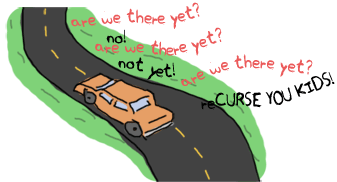
\includegraphics[width=1\linewidth]{reCURSE.png}
\end{wrapfigure}
Некоторые читатели, знакомые с императивными и объектно\--ориентированными языками программирования, должно быть, недоумевают, почему до сих пор не были показаны циклы.
Ответить на это можно вопросом: <<Что такое цикл?>>
По правде говоря, функциональные языки программирования обычно не предлагают средства построения циклов, такие как \ops{for} и \ops{while}.
Вместо них программисты\--функциональщики полагаются на незамысловатую концепцию, именуемую \emph{рекурсией}.

Вы, должно быть, помните как во вводной главе объяснялись неизменяемые переменные.
Если не помните, то уделите им \ref{invariable-variables}~ещё немного внимания!
Рекурсию тоже можно объяснить при помощи математических концепций и функций.
Хорошим примером функции, которую можно выразить в рекурсивном виде, может послужить примитивная функция вычисления факториала.
Факториал числа \emph{n} это произведение последовательности \ops{$1\times 2\times3\times\ldots\times\emph{n}$} или \ops{$n\times n-1 \times n-2\times\ldots\times 1$}.
Например, факториал числа 3 равен \ops{$3! = 3 \times 2 \times 1 = 6$}.
Факториал 4 равен \ops{$4! = 4 \times 3 \times 2 \times 1 = 24$}.
Эту функцию можно выразить при помощи математической записи в следующем виде:
\[
n! =
  \begin{cases}
   1           & \text{if } x = 0 \\
   n((n - 1)!) & \text{if } x < 0
  \end{cases}
\]

Это означает, что если n равно 0, то в качестве результата возвращается 1.
Для любого значения больше 0 возвращается \emph{n} умноженное на факториал \ops{n - 1}, значение которого тоже раскрывается, до тех пор, пока не достигнет 1.
\begin{align*}
4! &= 4 \times 3! \\
4! &= 4 \times 3 \times 2! \\
4! &= 4 \times 3 \times 2 \times 1! \\
4! &= 4 \times 3 \times 2 \times 1 \times 1 \\
\end{align*}

Как же записать такую математическую функцию на Erlang? Очень просто.
Взгляните на части записи: \ops{n!}, 1 и \ops{n((n-1)!)}, а затем на \ops{if}\--ы.
Мы можем различить имя функции (\ops{n!}), стражей (им соответствуют \ops{if}\--ы) и тело функции (1 и \ops{n((n-1)!)}).
Мы переименуем \ops{n!} в \ops{fac(N)}, чтобы немного ограничить наш синтаксис, и получим следующее:
\begin{lstlisting}[style=erlang]
-module(recursive).
-export([fac/1]).
 
fac(N) when N == 0 -> 1;
fac(N) when N > 0  -> N*fac(N-1).
\end{lstlisting}

Вот и готова наша функция для вычисления факториала!
Она очень похожа на математическое определение.
Применяя сопоставление с образцом, мы можем немного сократить её объявление:
\begin{lstlisting}[style=erlang]
fac(0) -> 1;
fac(N) when N > 0 -> N*fac(N-1).
\end{lstlisting}

Для математического определения, которое рекурсивно по своей природе, трансляция на Erlang происходит просто и быстро.
Мы записали цикл!
Определение рекурсивной функции можно сократить до <<функция, которая вызывает саму себя>>.
Также нам необходимо определить условие остановки вычислений (это называется базовым случаем), так как без такого условия мы будем находиться в цикле бесконечно.
В нашем примере условие остановки \--- это состояние, когда \emph{n} равно 0.
В момент, когда это условие истинно, мы перестаём вызывать функцию, и её исполнение прекращается. 
\section{Длина}
\label{length}
Попробуем перейти к более практичным вещам.
Напишем функцию, которая считает количество элементов, содержащихся в списке.
Сразу же ясно, что нам понадобится:\\
\begin{itemize}
\item базовый случай;
\item функция, которая вызывает сама себя;
\item список, к которому мы применим нашу функцию.
\end{itemize}

Мне кажется, что для большинства рекурсивных функций проще всего сначала записать базовый случай.
Что представляет собой самый простой входящий параметр, для которого мы можем найти длину?
Это, конечно же, пустой список, длина которого равна 0.
Поэтому запомним, что \ops{[] = 0}.
Следующий по простоте список имеет длину 1: \ops{[\_] = 1}.
Похоже, у нас есть всё необходимое, чтобы записать определение нашей функции:
\begin{lstlisting}[style=erlang]
len([]) -> 0;
len([_]) -> 1.
\end{lstlisting}

Прекрасно!
Мы можем подсчитать длину списка, если он содержит 0 либо 1 элемент!
Очень полезная возможность.
Правда, пользы в ней не так много, потому что ей не хватает рекурсивности.
Это приводит нас к самому сложному моменту: нам необходимо расширить функцию таким образом, чтобы она вызывала сама себя для списков с длиной больше 0 и 1.
Ранее мы \ref{lists}~упоминали, что списки определяются рекурсивно как \ops{[1 | [2| \ldots [n| []]]]}.
Это означает, что мы можем использовать образец \ops{[H|T]} для сопоставления со списками одного и более элементов, так как список с одним элементом можно определить как \ops{[X|[]]}, а список с двумя элементами как \ops{[X|[Y|[]]]}.
Обратите внимание, что второй элемент сам является списком.
Поэтому нам нужно посчитать лишь первый элемент, а потом функция может вызвать себя для второго элемента.
Если учесть, что каждый элемент в списке прибавляет к длине 1, то функцию можно переписать в следующем виде:
\begin{lstlisting}[style=erlang]
len([]) -> 0;
len([_|T]) -> 1 + len(T).
\end{lstlisting}

Вот у нас и появилась рекурсивная функция, которая определяет длину списка.
Давайте посмотрим как она будет вести себя при исполнении. Попробуем применить её, например, к списку \ops{[1,2,3,4]}: \begin{align*}
len([1,2,3,4]) &= len([1 | [2,3,4])\\
&= 1 + len([2 | [3,4,]])\\
&= 1 + 1 + len([3 | [4]])\\
&= 1 + 1 + 1 + len([4 | []])\\
&= 1 + 1 + 1 + 1 + len([])\\
&= 1 + 1 + 1 + 1 + 0\\
&= 1 + 1 + 1 + 1\\
&= 1 + 1 + 2\\
&= 1 + 3\\
&= 4
\end{align*}
Мы получили верный результат.
Поздравляю вас с первой полезной рекурсивной функцией на Erlang!
\section{Длина хвостовой рекурсии}
\label{length-of-a-tail-recursion}

\begin{wrapfigure}{l}{0.4\linewidth}
    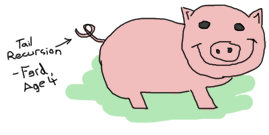
\includegraphics[width=1\linewidth]{tail-recursion.png}
\end{wrapfigure}
Возможно, вы заметили, что для списка из четырёх термов, мы разложили вызов нашей функций на цепь из пяти операций суммирования.
Хотя этот принцип хорошо работает для коротких списков, он может создать проблемы для случая, когда ваш список содержит несколько миллионов значений.
Для такого простого вычисления совсем не обязательно хранить в памяти миллионы чисел.
Это слишком расточительно, к тому же, есть способ получше.
Познакомьтесь с \emph{хвостовой рекурсией}.

Хвостовая рекурсия \--- это способ трансформации вышеописанного линейного процесса (который растёт прямо пропорционально количеству элементов) в итеративный (в котором никакого роста нет вообще).
Чтобы вызов функции стал хвостовым, он должен быть <<одиночным>>.
Здесь необходимо пояснить: наши предыдущие вызовы росли из\--за того, что результат первого вызова зависел от вычисления второго.
Чтобы найти ответ для \ops{1 + len(Rest)}, необходимо вычислить результат \ops{len(Rest)}.
А для вычисления \ops{len(Rest)}, в свою очередь, понадобится найти результат ещё одного вызова функции.
Операции суммирования будут накапливаться до тех пор, пока не будет найден результат последней, и только после этого можно будет вычислить конечный результат.
Хвостовая рекурсия позволяет избавиться от этого накопления посредством вычисления операций по мере их возникновения.

Чтобы этого добиться, нам необходимо завести временную переменную и передавать её при каждом вызове функции в качестве дополнительного параметра.
Я проиллюстрирую эту концепцию при помощи функции вычисления факториала.
На этот раз определим её с использованием хвостовой рекурсии.
Вышеупомянутую временную переменную иногда называют \emph{аккумулятором}.
Для ограничения роста вызовов нашей функции, мы сохраняем в аккумуляторе результаты вычислений, по мере того как они происходят:
\begin{lstlisting}[style=erlang]
tail_fac(N) -> tail_fac(N,1).
 
tail_fac(0,Acc) -> Acc;
tail_fac(N,Acc) when N > 0 -> tail_fac(N-1,N*Acc).
\end{lstlisting}

Я определил две функции \ops{tail\_fac/1} и \ops{tail\_fac/2}.
Сделал я это по причине того, что Erlang не позволяет указывать для параметров значения по умолчанию (функции c разной арностью, которые имеют одинаковые имена \--- это разные функции), поэтому мы создаём аналогичный эффект вручную.
В данном случае \ops{tail\_fac/1} реализует абстракцию поверх функции \ops{tail\_fac/2}, которая использует хвостовую рекурсию.
Никого не интересуют детали реализации скрытого аккумулятора, который использует \ops{tail\_fac/2}, поэтому мы будем экспортировать из модуля лишь \ops{tail\_fac/1}.
Исполнение функции можно записать в следующем виде:
\begin{align*}
tail\_fac(4) &= tail\_fac(4,1)\\
tail\_fac(4,1) &= tail\_fac(4-1, 4*1)\\
tail\_fac(3,4) &= tail\_fac(3-1, 3*4)\\
tail\_fac(2,12) &= tail\_fac(2-1,2*12)\\
tail\_fac(1,24) &= tail\_fac(1-1, 1*24)\\
tail\_fac(0,24) &= 24
\end{align*}

Видите разницу?
Теперь нам не нужно держать в памяти одновременно более двух термов.
Количество места, выделяемого под хранение данных, не меняется.
Для вычисления факториала числа 4 понадобится столько же места, сколько для вычисления факториала 1000000 (если не учитывать, что 4! занимает в числовом представлении намного меньше места, чем 1000000!).

Теперь, когда вы видели функцию вычисления факториала с использованием хвостовой рекурсии, вам, наверняка, ясно как этот шаблон можно применить к нашей функции \ops{len/1}.
Необходимо лишь сделать так, чтобы к результату рекурсивного вызова больше не применялись никакие операции.
Для тех, кто любит визуальные примеры, представьте, что вы помещаете операцию \ops{+1} внутрь вызова функции путём добавления к параметру:
\begin{lstlisting}[style=erlang]
len([]) -> 0;
len([_|T]) -> 1 + len(T).
\end{lstlisting}
принимает вид:
\begin{lstlisting}[style=erlang]
tail_len(L) -> tail_len(L,0).
 
tail_len([], Acc) -> Acc;
tail_len([_|T], Acc) -> tail_len(T,Acc+1).
\end{lstlisting}

Теперь ваша функция вычисления длины списка использует хвостовую рекурсию.
\section{Снова рекурсивные функции}
\begin{wrapfigure}{l}{0.3\linewidth}
    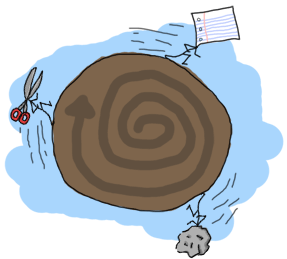
\includegraphics[width=1\linewidth]{rock-paper-scissors.png}
\end{wrapfigure}
Чтобы немного привыкнуть к рекурсивным функциям, мы напишем ещё несколько.
В конце концов, рекурсия \--- это единственный способ организации итераций, который существует в Erlang (кроме списковых выражений), поэтому эту концепцию очень важно понимать.
Это знание будет также полезно для любого другого функционального языка программирования, с которым вы можете столкнуться позже, поэтому запоминайте!

Первая функция, которую мы напишем \--- \ops{duplicate/2}.
Она принимает первым параметром целое число, а вторым \--- произвольный терм.
Затем она создаёт список, который содержит столько копий терма, сколько указано в первом параметре.
Как и ранее, для начала неплохо подумать о базовом случае.
Самое простое, что может сделать функция \ops{duplicate/2}, это повторить что\--либо 0 раз.
Для этого она должна просто возвратить пустой список, не учитывая передаваемый терм.
В любом другом случае мы должны пытаться добраться до базового путём рекурсивного вызова функции.
Вдобавок, мы запретим целому параметру принимать отрицательные значения, потому что нельзя повторить что\--либо \ops{-n} раз:
\begin{lstlisting}[style=erlang]
duplicate(0,_) ->
    [];
duplicate(N,Term) when N > 0 ->
    [Term|duplicate(N-1,Term)].
\end{lstlisting}

Как только мы определили основную рекурсивную функцию, её становится проще записать в виде, который использует хвостовую рекурсию.
Делается это путём перемещения операции создания списка во временную переменную:
\begin{lstlisting}[style=erlang]
tail_duplicate(N,Term) ->
    tail_duplicate(N,Term,[]).
 
tail_duplicate(0,_,List) ->
    List;
tail_duplicate(N,Term,List) when N > 0 ->
    tail_duplicate(N-1, Term, [Term|List]).
\end{lstlisting}

Получилось!
Теперь я хотел бы немного изменить предмет обсуждения, чтобы обозначить связь между хвостовой рекурсией и циклом while.
Наша функция \ops{tail\_duplicate/2} содержит все части, которые присущи циклу while.
Если бы мы представили себе цикл while в выдуманном языке с синтаксисом похожим на Erlang, то наша функция могла бы выглядеть следующим образом:
\begin{lstlisting}[style=erlang]
function(N, Term) ->
    while N > 0 ->
        List = [Term|List],
        N = N-1
    end,
    List.
\end{lstlisting}

Обратите внимание, что все элементы цикла присутствуют как в воображаемом языке, так и в Erlang.
Отличается лишь их расположение.
Это показывает, что правильно написанная функция, использующая хвостовую рекурсию, подобна итеративному процессу, такому как цикл while.

Есть также ещё одно интересное свойство, которое мы <<откроем>> путём сравнении рекурсивной функции и функции с хвостовой рекурсией.
Мы напишем функцию \ops{reverse/1}, которая будет разворачивать список термов задом\--наперёд.
Базовым случаем в этой функции является пустой список, для которого разворачивать нечего.
Для пустого списка мы можем просто вернуть пустой список.
В любой другой ситуации функция должна сходиться к базовому случаю, вызывая саму себя, как это было в \ops{duplicate/2}.
Наша функция будет перебирать элементы списка при помощи сопоставления с образцом \ops{H|T]}, а потом добавлять \emph{H} в конец списка:
\begin{lstlisting}[style=erlang]
reverse([]) -> [];
reverse([H|T]) -> reverse(T)++[H].
\end{lstlisting}

Для длинных списков это может оказаться настоящим кошмаром: помимо проблемы наслаивания функций добавления, нам придётся для каждой операции добавления в конец списка проходить список полностью от начала до конца!
Визуально это можно представить как:
\begin{align*}
reverse([1,2,3,4]) &= [4]++[3]++[2]++[1]\\
&= [4,3]++[2]++[1]\\
&= [4,3,2]++[1]\\
&= [4,3,2,1]\\
\end{align*}

На помощь к нам приходит хвостовая рекурсия.
Мы будем добавлять к аккумулятору новый головной элемент на каждой итерации.
Это автоматически развернёт список в противоположном направлении.
Посмотрим на реализацию:
\begin{lstlisting}[style=erlang]
tail_reverse(L) -> tail_reverse(L,[]).
 
tail_reverse([],Acc) -> Acc;
tail_reverse([H|T],Acc) -> tail_reverse(T, [H|Acc]).
\end{lstlisting}

Если мы распишем шаги исполнения этой функции, то получим:
\begin{align*}
tail\_reverse([1,2,3,4]) &= tail\_reverse([2,3,4], [1])\\
&= tail\_reverse([3,4,], [2,1])\\
&= tail\_reverse([4], [3,2,1])\\
&= tail\_reverse([], [4,3,2,1])\\
&= [4,3,2,1]
\end{align*}

Можно заметить, что теперь мы посещаем линейное количество элементов.
Наш стек не будет расти, и эффективность выполнения операций добавления элементов в этом случае намного выше!

Реализуем ещё одну функцию \--- \ops{sublist/2}. Она принимает список \emph{L} и целое число \emph{N}, и возвращает первых \emph{N} элементов из списка.
Например, вызов \ops{sublist([1,2,3,4,5,6],3)} возвратит [1,2,3].
И снова базовый случай \--- попытка получить 0 элементов из списка.
Впрочем, будьте осторожны, так как в случае \ops{sublist/2} есть отличия.
Есть и второй базовый случай, в котором передаётся пустой список!
Если мы не сделаем проверку списка на пустоту, то при вызове \ops{recursive:sublist([1],2).} будет выброшена ошибка, хотя в качестве результата мы ожидали получить \ops{[1]}.
Как только мы разобрались с этими проблемами, рекурсивной части функции остаётся лишь пройти по списку, сохраняя элементы до тех пор, пока она не упрётся в один из базовых случаев:
\begin{lstlisting}[style=erlang]
sublist(_,0) -> [];
sublist([],_) -> [];
sublist([H|T],N) when N > 0 -> [H|sublist(T,N-1)].
\end{lstlisting}

Функцию можно привести к форме с использованием хвостовой рекурсии тем же путём, что и прежде:
\begin{lstlisting}[style=erlang]
tail_sublist(L, N) -> tail_sublist(L, N, []).
 
tail_sublist(_, 0, SubList) -> SubList;
tail_sublist([], _, SubList) -> SubList;
tail_sublist([H|T], N, SubList) when N > 0 ->
tail_sublist(T, N-1, [H|SubList]).
\end{lstlisting}

Но в этой функции есть изъян.
Роковой изъян!
Мы используем в качестве аккумулятора список, так же как мы это делали, когда разворачивали список задом\--наперёд.
Если вы сейчас скомпилируете функцию, то вызов \ops{sublist([1,2,3,4,5,6],3)} возвратит не [1,2,3], а [3,2,1].
Поэтому нам нужно взять окончательный результат и развернуть его самостоятельно.
Просто поменяйте вызов \ops{tail\_sublist/2}, а рекурсивную логику оставьте прежней:
\begin{lstlisting}[style=erlang]
tail_sublist(L, N) -> reverse(tail_sublist(L, N, [])).
\end{lstlisting}

Окончательный результат будет упорядочен правильно.
Может показаться, что разворот списка после вызова хвостовой рекурсии \--- напрасная потеря времени, и это отчасти правда (таким образом мы всё равно экономим память).
Вы сможете заметить, что из\--за необходимости разворота, на коротких списках ваш код с использованием обычной рекурсии работает быстрее, чем код с хвостовой рекурсией.
Но по мере увеличения объёма данных, на фоне остальных операций разворачивание списка будет значить всё меньше и меньше.\\
\colorbox{lgray}
{
    \begin{minipage}{\linewidth}
\textbf{Замечание:} вместо собственноручно написанной функции \ops{reverse/1} вы должны использовать \ops{lists:reverse/1}.
Функция так часто использовалась для вызовов с хвостовой рекурсией, что разработчики Erlang решили превратить её во встроенную.
Списки будут разворачиваться чрезвычайно быстро (благодаря тому, что функция написана на языке C), что сделает замедление, которое вносит разворот, менее заметным.
Остальной код в этой главе будет использовать нашу собственную функцию разворота элементов, но больше вы её никогда использовать не должны.
    \end{minipage}
}

Чтобы немного развить тему, мы напишем zip\--функцию.
Такая функция принимает в качестве параметров два списка одинаковой длины и попарно комбинирует их элементы в виде списка кортежей.
Наша функция \ops{zip/2} будет вести себя следующим образом:
\begin{lstlisting}[style=erlang]
1> recursive:zip([a,b,c],[1,2,3]).
[{a,1},{b,2},{c,3}]
\end{lstlisting}

Так как мы хотим, чтобы оба параметра имели одинаковую длину, нашим базовым случаем будет комбинирование двух пустых списков:
\begin{lstlisting}[style=erlang]
zip([],[]) -> [];
zip([X|Xs],[Y|Ys]) -> [{X,Y}|zip(Xs,Ys)].
\end{lstlisting}

Однако, если вы хотите, чтобы функция мягче относилась к параметрам, лучше позволить ей заканчивать обработку, когда опустеет один из списков.
Для такого сценария у вас появится два базовых случая:
\begin{lstlisting}[style=erlang]
lenient_zip([],_) -> [];
lenient_zip(_,[]) -> [];
lenient_zip([X|Xs],[Y|Ys]) -> [{X,Y}|lenient_zip(Xs,Ys)].
\end{lstlisting}

Обратите внимание, что вне зависимости от того, какие мы определяем базовые случаи, рекурсивная часть функции остаётся неизменной.
Я бы посоветовал вам попробовать написать собственные версии \ops{zip/2} и \ops{lenient\_zip/2} с использованием хвостовой рекурсии, чтобы убедиться, что вы полностью понимаете как создаются такие функции.
Хвостовая рекурсия будет одной из центральных концепций, лежащих в основе большого приложения, главный цикл которого будет организован именно таким образом.

Если хотите проверить то, что у вас получилось, взгляните на мою реализацию в \href{http://learnyousomeerlang.com/static/erlang/recursive.erl}{recursive.erl}, а именно на функции \ops{tail\_zip/2} и \ops{tail\_lenient\_zip/3}.
\colorbox{lgray}
{
    \begin{minipage}{\linewidth}
\textbf{Замечание:} хвостовая рекурсия не раздувает используемую память, так как виртуальная машина видит, что рекурсивный вызов происходит из хвостовой позиции (последнее выражение, которое обрабатывает функция), и устраняет текущий стековый кадр.
Эта техника называется оптимизацией хвостового вызова и является специальным случаем более общей оптимизации под названием \emph{оптимизация последнего вызова}.\\
Оптимизация последнего вызова происходит, когда последнее выражение в теле функции является ещё одним вызовом функции.
В этом случае, как и в случае оптимизации хвостовой рекурсии, виртуальная машина Erlang не сохраняет стековый кадр.
Поэтому хвостовая рекурсия возможна между несколькими функциями.
Например, цепь функций \ops{a() -> b(). b() -> c(). c() -> a().} создаст в результате бесконечный цикл, который не приведёт к исчерпанию памяти, так как оптимизация последнего вызова предотвращает переполнение стека.
Этот принцип в сочетании с использованием аккумуляторов делает хвостовую рекурсию полезной техникой.
    \end{minipage}
}
\section{Быстро, сортируй!}
\begin{wrapfigure}{l}{0.4\linewidth}
    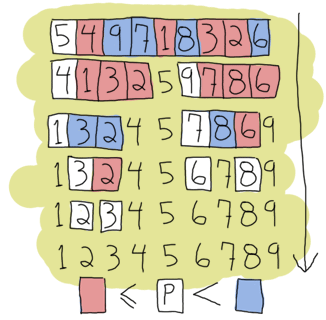
\includegraphics[width=1\linewidth]{quicksort.png}
\end{wrapfigure}
Я могу (и буду) считать, что рекурсия и хвостовая рекурсия вам ясна.
Но просто чтобы в этом убедиться, я приведу более сложный пример \--- реализацию алгоритма быстрой сортировки.
Да, традиционный <<эй, смотри, я могу писать сжатый функциональный код>> канонический пример.
Наивная реализация алгоритма быстой сортировки выбирает первый элемент списка, \emph{опорный элемент}, и перемещает все элементы меньшие, либо равные опорному элементу в новый список, а все элементы больше опорного элемента \--- в другой список.
Затем мы повторяем эту процедуру для полученных списков.
Этот процесс продложается до тех пор, пока для сортировки не останется ничего, кроме пустых списков, которые и станут нашим базовым случаем.
Эта реализация считается простой, потому что более эффективные версии быстрой сортировки будут пытаться выбрать оптимальные опорные элементы с целью ускорения.
Впрочем, в нашем примере это не столь важно.

Нам понадобятся две функции: первая будет разбивать список на части, содержащие меньшие и большие элементы, а вторая будет применять функцию разбиения к новым спискам и соединять их в единое целое.
Для начала мы напишем функцию соединения:
\begin{lstlisting}[style=erlang]
quicksort([]) -> [];
quicksort([Pivot|Rest]) ->
{Smaller, Larger} = partition(Pivot,Rest,[],[]),
quicksort(Smaller) ++ [Pivot] ++ quicksort(Larger).
\end{lstlisting}

Здесь мы видим: базовый случай; список, который разбит при помощи ещё одной функции на части с большими и меньшими элементами; опорный элемент, к которому слева и справа присоединены отсортированные списки.
Этот код отвечает за соединение списков.
Перейдём к функции разбиения:
\begin{lstlisting}[style=erlang]
partition(_,[], Smaller, Larger) -> {Smaller, Larger};
partition(Pivot, [H|T], Smaller, Larger) ->
    if H =< Pivot -> partition(Pivot, T, [H|Smaller], Larger);
        H >  Pivot -> partition(Pivot, T, Smaller, [H|Larger])
    end.
\end{lstlisting}

Теперь функцию быстрой сортировки можно запустить.
Если вы искали в Интернет примеры программ на Erlang, то, скорее всего, наталкивались на другую реализацию быстрой сортировки, ту, которая выглядит проще и легче читается, но использует списковые выражения.
Их легко можно применить в месте, где создаются новые списки, в функции \ops{partition/4}:
\begin{lstlisting}[style=erlang]
lc_quicksort([]) -> [];
lc_quicksort([Pivot|Rest]) ->
    lc_quicksort([Smaller || Smaller <- Rest, Smaller =< Pivot])
    ++ [Pivot] ++
    lc_quicksort([Larger || Larger <- Rest, Larger > Pivot]).
\end{lstlisting}

Главное отличие этой версии в том, что её код легче читать, но за лёгкость чтения приходится платить тем, что для разбиения списка, необходимо перебрать все его элементы.
В этом проявляется борьба ясности кода против скорости его исполнения.
Но проигрываете в этой борьбе лишь вы, потому что для таких ситуаций уже создана функция \ops{lists:sort/1}.
Используйте лучше её.\\
\colorbox{lorange}
{
    \begin{minipage}{1.0\linewidth}
\textbf{Не забывайтесь:}\\
Выразительность кода хороша для обучения, но не всегда полезна для производительности.
Множество руководств по функциональному программированию ни слова об этом не говорят!
Во\--первых, обеим реализациям, приведённым здесь, приходится неоднократно обрабатывать элементы равные опорному элементу.
Для увеличения эффективности можно было бы возвращать три списка: элементы меньше, больше и равные опорному элементу.\\
Ещё одна проблема связана с тем, что нам необходимо неоднократно проходить по разбитым спискам при их слиянии с опорным элементом.
Можно немного уменьшить накладные расходы, если производить объединение во время разбиения списков на три части.
Тем, кто заинтересовался реализацией, я предлагаю взглянуть на последнюю функцию (\ops{bestest\_qsort/1}) из файла \href{http://learnyousomeerlang.com/static/erlang/recursive.erl}{recursive/erl}.\\
Приятно отметить, что все рассмотренные реализации быстрой сортировки будут работать со списками, содержащими любые типы, даже кортежи или что\--то подобное.
Попробуйте, они работают!
    \end{minipage}
}
\section{Больше чем списки}
\begin{wrapfigure}{l}{0.4\linewidth}
    
\includegraphics[width=1\linewidth]{tree.png}
\end{wrapfigure}
Читая эту главу, вы, возможно, начинаете думать, что рекурсия в Erlang, главным образом, связана со списками.
Хотя списки и могут служить хорошим примером структуры, которую можно определить через рекурсию, но на ней, конечно, всё не заканчивается.
Мы рассмотрим, для разнообразия, как можно создавать двоичные деревья и считывать из них данные.

Для начала неплохо было бы определить, что такое дерево.
В нашем случае оно снизу доверху состоит из узлов.
Узлы \--- это кортежи, которые содержат ключ, данные связанные с ключом, и два других узла.
Эти два узла мы разделяем на узел с ключом меньшим и большим, чем ключ узла, который их содержит.
И вот появляется рекурсия!
Дерево \--- это узел, который содержит узлы, каждый из которых содержит узлы, которые, в свою очередь, содержат узлы.
Бесконечно это не может продолжаться (у нас нет бесконечного пространства для хранения данных), поэтому мы скажем, что узлы, которые содержатся в наших узлах, также могут быть пустыми.

Кортежи \--- подходящая структура для представления узлов.
Для нашей реализации мы определим такие кортежи как \ops{\{node, \{Key, Value, Smaller, Larger\}\}} (меченый кортеж!), где \emph{Smaller} и \emph{Larger} могут быть другим подобным узлом, или пустым узлом (\ops{\{node, nil\}}.
Более сложные концепции нам не понадобятся.

Начнём создавать модуль для нашей \href{http://learnyousomeerlang.com/static/erlang/tree.erl}{очень простой реализации дерева}.
Первая функция \ops{empty/0} \--- возвращает пустой узел.
Пустой узел \--- это начальная точка нового дерева, которая также называется \emph{корневым узлом}:
\begin{lstlisting}[style=erlang]
-module(tree).
-export([empty/0, insert/3, lookup/2]).
 
empty() -> {node, 'nil'}.
\end{lstlisting}

Мы скрываем реализацию, используя эту функцию, и, затем, инкапсулируем её в одинаковое представление узлов, чтобы пользователю не пришлось задумываться о том, как устроен наш код.
Вся эта информация будет существовать лишь в рамках модуля.
Если вам когда\--либо придёт в голову изменить представление узла \--- вы сможете сделать изменения, не нарушая работу внешнего кода.

Для того, чтобы наполнить дерево содержимым, нам необходимо, для начала, понять, как по нему рекурсивно перемещаться.
Давайте поступим так же, как мы поступали в любом другом примере с рекурсией \--- попытаемся найти базовый случай.
Так как пустое дерево состоит из пустого узла, то, рассуждая логически, нашим базовым случаем будет пустой узел.
Мы сможем добавить новую пару ключ/значение, когда наткнёмся на пустой узел.
В остальных случаях наш код будет ходить по дереву в поисках пустого узла, который можно наполнить данными.

Мы будем искать пустой узел, начиная с корневого узла.
Для этого мы должны использовать знание о том, что \emph{Меньший} и \emph{Больший} узлы позволяют нам определять направление перемещения, сравнивая новый ключ, который необходимо добавить, с ключом текущего узла.
Если новый ключ меньше ключа текущего узла, то мы продолжаем искать пустой узел внутри \emph{Меньшего} узла, и если больше, то внутри \emph{Большего}.
Нельзя забывать ещё об одном случае: что будет, если новый ключ равен ключу текущего узла?
У нас есть две возможности: сгенерировать ошибку, либо заменить значение узла новым.
Здесь мы используем замену.
Все эти рассуждения, заключённые в код, выглядят следующим образом:
\begin{lstlisting}[style=erlang]
insert(Key, Val, {node, 'nil'}) ->
    {node, {Key, Val, {node, 'nil'}, {node, 'nil'}}};
insert(NewKey, NewVal, {node, {Key, Val, Smaller, Larger}}) when NewKey < Key ->
    {node, {Key, Val, insert(NewKey, NewVal, Smaller), Larger}};
insert(NewKey, NewVal, {node, {Key, Val, Smaller, Larger}}) when NewKey > Key ->
    {node, {Key, Val, Smaller, insert(NewKey, NewVal, Larger)}};
insert(Key, Val, {node, {Key, _, Smaller, Larger}}) ->
    {node, {Key, Val, Smaller, Larger}}.
\end{lstlisting}

Обратите внимание, что функция возвращает совершенно новое дерево.
Это характерная черта функциональных языков программирования, в которых присваивание происходит лишь один раз.
Хотя это и может показаться неэффективным, но большая часть структур, которые лежат в основе обеих версий дерева, остаются теми же и используются совместно, а поэтому копируются виртуальной машиной лишь по необходимости.

Для завершения этой демонстрационной реализации дерева, нам необходимо создать функцию \ops{lookup/2}, которая позволит найти значение узла по ключу.
Мы будем использовать принцип, чрезвычайно похожий на тот, который мы использовали при добавлении новых данных в дерево: мы проходим по узлам дерева, шаг за шагом проверяя, что искомый ключ больше, меньше, либо равен ключу текущего узла.
У нас есть два базовых случая: первый \--- когда узел пуст (ключа в дереве нет), и второй \--- когда ключ найден.
Мы не хотим, чтобы наша программа сбоила каждый раз, когда мы ищем ключ, который в дереве отсутствует, а поэтому в такой ситуации мы будем возвращать атом 'undefined'.
В случае удачи, мы возвращаем \ops{\{ok, Value\}}.
Если бы мы просто возвращали \emph{Value}, а искомый узел содержал атом 'undefined', то мы не могли бы понять, было найдено верное значение или нет.
Обёртывание успешно найденных результатов позволяет их легко отличать от неудачных.
Вот реализация функции:
\begin{lstlisting}[style=erlang]
lookup(_, {node, 'nil'}) ->
    undefined;
lookup(Key, {node, {Key, Val, _, _}}) ->
    {ok, Val};
lookup(Key, {node, {NodeKey, _, Smaller, _}}) when Key < NodeKey ->
    lookup(Key, Smaller);
lookup(Key, {node, {_, _, _, Larger}}) ->
    lookup(Key, Larger).
\end{lstlisting}

Всё, мы закончили.
Давайте потестируем нашу структуру \--- напишем небольшую адресную книгу для электронной почты.
Скомпилируйте файл и запустите оболочку:
\begin{lstlisting}[style=erlang]
1> T1 = tree:insert("Jim Woodland", "jim.woodland@gmail.com", tree:empty()).
{node,{"Jim Woodland","jim.woodland@gmail.com",
    {node,nil},
    {node,nil}}}
2> T2 = tree:insert("Mark Anderson", "i.am.a@hotmail.com", T1).
{node,{"Jim Woodland","jim.woodland@gmail.com",
    {node,nil},
    {node,{"Mark Anderson","i.am.a@hotmail.com",
        {node,nil},
        {node,nil}}}}}
3> Addresses = tree:insert("Anita Bath", "abath@someuni.edu", tree:insert("Kevin Robert", "myfairy@yahoo.com", tree:insert("Wilson Longbrow", "longwil@gmail.com", T2))).
{node,{"Jim Woodland","jim.woodland@gmail.com",
    {node,{"Anita Bath","abath@someuni.edu",
        {node,nil},
        {node,nil}}},
    {node,{"Mark Anderson","i.am.a@hotmail.com",
        {node,{"Kevin Robert","myfairy@yahoo.com",
            {node,nil},
            {node,nil}}},
        {node,{"Wilson Longbrow","longwil@gmail.com",
            {node,nil},
            {node,nil}}}}}}}
\end{lstlisting}

Теперь можно поискать адреса с помощью нашей книги:
\begin{lstlisting}[style=erlang]
4> tree:lookup("Anita Bath", Addresses).
{ok, "abath@someuni.edu"}
5> tree:lookup("Jacques Requin", Addresses).
undefined
\end{lstlisting}

На этом мы завершаем рассмотрение примера функциональной адресной книги, построенной при помощи рекурсивной структуры данных отличной от списка!\\
\colorbox{lgray}
{
    \begin{minipage}{\linewidth}
\textbf{Замечание:} наша реализация весьма примитивна: мы не поддерживаем часто используемые операции, такие как удаление узлов или перебалансировка дерева для ускорения последующих операций поиска.
Если вам интересно было бы реализовать и/или изучить эти операции \--- обратитесь к реализации модуля \ops{gb\_trees} (\ops{otp\_src\_R<version>B<revision>/lib/stdlib/src/gb\_trees.erl}).
Кроме того, при работе с деревьями используйте именно этот модуль и не пытайтесь изобрести велосипед.
    \end{minipage}
}
\section{Рекурсивное мышление}
Если вы поняли всё сказанное в этой главе, то рекурсивное мышление, вероятно, начинает становиться частью вашей интуиции.
Главное отличие рекурсивных определений от их императивных аналогов (обычно это циклы while или for) в том, что вместо пошагового выполнения (<<сделай это, потом то, затем вот это, после этого заверши исполнение>>) мы используем декларативный подход (<<если ты получишь такой входящий параметр, сделай это, в противном случае \--- вот это>>).
Такое свойство становится более очевидным при использовании сопоставления с образцом в заголовке функции.

Если вы до сих пор не поняли как работает рекурсия, может быть вам нужно прочитать вот \ref{recursion}~это.

Отбросив шутки в сторону, нужно признать, что иногда рекурсия в сочетании с сопоставлением с образцом \--- это оптимальный способ записи ясных и понятных алгоритмов.
После того как каждая часть задачи поделена на функции, которые не поддаются дальнейшему упрощению, алгоритм превращается в компоновку правильных ответов, получаемых из коротких подпрограмм (что\--то подбное мы делали с быстрой сортировкой).
С обычными циклами можно тоже использовать такой тип мысленной абстракции, но на практике это получается лучше именно с рекурсией.
Ваш опыт может свидетельствовать об ином.

\textbf{А теперь, леди и джентльмены \--- дискуссия автора с самим собой}

\--- Хорошо, кажется я понял рекурсию.
Я понимаю, что она связана с декларативностью, что корни её уходят в математику, как и у неизменяемых переменных. Я понимаю, что в некоторых случаях её проще использовать. Что ещё?

\--- Она имеет регулярную структуру.
Найди базовый случай, запиши его.
Для получения результата нужно, чтобы любой другой случай сходился к одному из базовых.
Так проще записывать функции.

\--- Ага, понял, ты это уже говорил несколько раз.
Я то же самое могу сделать циклами.

\--- Да, можешь.
Не буду отрицать!

\--- Хорошо.
Мне не совсем ясно, зачем ты писал функции, которые не используют хвостовую рекурсию, раз уж они намного хуже тех, что её используют.

\--- А, ну это просто чтобы было легче понять.
Мне показалось, что переход от обычный рекурсии, которая выглядит красивее и проще для понимания, к хвостовой рекурсии, которая теоретически более эффективна, неплохо показал все плюсы и минусы этих подходов.

\--- Хорошо, значит ни для чего кроме обучения они не годятся, я понял.
\begin{wrapfigure}{r}{0.4\linewidth}
    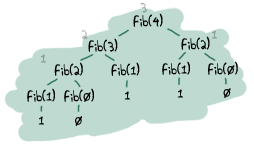
\includegraphics[width=1\linewidth]{fib.png}
\end{wrapfigure}

\--- Это не совсем так.
Разница в производительности между функцией с хвостовой рекурсией и обычной рекурсией будет не сильно заметна.
Хвостовая рекурсия хорошо подходит для функций, которые итерируют бесконечно, например для главных циклов.
Есть также функции, которые порождают очень большой стековый кадр, медленно исполняются и, если их не записывать в виде хвостовой рекурсии, могут рано приводить к аварийному завершению.
Неплохим примером может служить задача вычисления \href{http://en.wikipedia.org/wiki/Fibonacci\_number}{чисел Фибоначчи}, сложность которой растёт экспоненциально, если не решать её в виде итеративного процесса или хвостовой рекурсии.
Также необходимо профилировать написанный код (позже я покажу как это делать, я обещаю), определять и исправлять места, которые замедляют исполнение.

\--- Но циклы \--- это всегда итеративный процесс, проще использовать их и не знать проблем.

\--- Да, но\ldots но\ldots мой прекрасный Erlang\ldots

\--- Ну, зашибись.
Весь сыр\--бор из\--за того, что в Erlang нет <<while>> и <<for>>.
Спасибо большое, я пошёл дальше программировать свой тостер на C!

\--- Погоди\--ка!
У функциональных языков программирования есть и другие возможности!
Кроме шаблона для поиска базовых случаев, который облегчил нам жизнь при написании рекурсивных функций, существует ещё много других шаблонов, которые придумали умные люди.
Благодаря этому необходимость самостоятельно писать рекурсивные функции значительно уменьшается.
Если ты продолжишь занятия, я покажу как строить такие абстракции.
Но для этого нам нужно взять что\--то помощнее.
Позволь мне рассказать о функциях высшего порядка\ldots
